\documentclass{article}
% translate with >> pdflatex -shell-escape <file>

% This file is used as unit test for pgfplots, copyright by Christian Feuersaenger.
% 
% See
%   http://pgfplots.sourceforge.net/pgfplots.pdf
% for pgfplots.
%
% Any required input files (for <plot table> or <plot file> or the table package) can be downloaded
% at
% http://www.ctan.org/tex-archive/graphics/pgf/contrib/pgfplots/doc/latex/
% and
% http://www.ctan.org/tex-archive/graphics/pgf/contrib/pgfplots/doc/latex/plotdata/

\usepackage{pgfplots}
\pgfplotsset{compat=newest}

\pagestyle{empty}

\def\smallplotstest{%
	\addplot[smooth,blue,mark=*] coordinates {
		(-1,	1)
		(-0.75,	0.5625)
		(-0.5,	0.25)
		(-0.25,	0.0625)
		(0,		0)
		(0.25,	0.0625)
		(0.5,	0.25)
		(0.75,	0.5625)
		(1,		1)
	};
}

\begin{document}

The following figure is centered:
\setlength{\fboxsep}{0pt}%
\begin{center}
\fbox{%
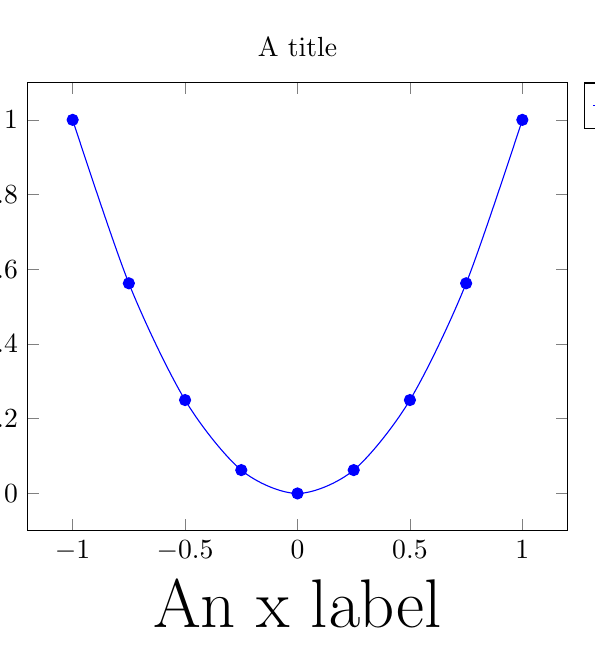
\begin{tikzpicture}%
	\begin{pgfinterruptboundingbox}
	\pgfplotsset{every axis legend/.append style={at={(1.03,1)},anchor=north west}}
	\begin{axis}[
		name=my plot,
		title=A title,
		xlabel={\Huge An x label},
		ylabel={$\displaystyle\sum_{k=1}^n \frac 1n$}
	]
		\smallplotstest
		\addlegendentry{My plot}
	\end{axis}
	\end{pgfinterruptboundingbox}

	\useasboundingbox (my plot.below south west) rectangle (my plot.above north east);
\end{tikzpicture}
}%
\end{center}
\end{document}
